\documentclass[conference]{IEEEtran}
\usepackage{graphicx}
\begin{document}
	\title{A Neural Network and Linear Model Approach Towards Performance Prediction For Secondary School Students}
    	\author{\IEEEauthorblockN{Anush S. Kumar\IEEEauthorrefmark{1},
					  Sreedhar Radhakirshnan\IEEEauthorrefmark{2} and
					  Sushrith Shriniwas Arkal\IEEEauthorrefmark{3}}
		\IEEEauthorblockA{Department of Computer Science and Engineering\\
					PES University, Bangalore\\
					Karnataka, India 560085\\
		USN:  \IEEEauthorrefmark{1}01FB14ECS037,
			\IEEEauthorrefmark{2}01FB14ECS247,
			\IEEEauthorrefmark{3}01FB14ECS262\\
		Email:  \IEEEauthorrefmark{1}anushkumar27@gmail.com,
			\IEEEauthorrefmark{2}sreedhar1895@gmail.com,
			\IEEEauthorrefmark{3}sushrith.arkal@gmail.com}}

	% make the title area
	\maketitle
	\pagenumbering{arabic}
	%--------------------------------------------------------------------------- Abstract----------------------------------------------------------------------------------
	\begin{abstract}
In this project we introduce a neural network and linear model approach to predict performance of students studying in secondary school. The practice of examining large pre-existing databases in order to generate new information helps us predict the outcomes with some certainty. With the help of such outcomes it is easy to make some hard decisions easily and also to plan the future events, one such application is the aim of this project. We are using around 10 attributes of different category that are not only academical in nature but also taking into account the socio-demographic condition of the student into the picture. 
%All this was possible with the data available in the UCI Machine Learning Repository's Student Performance Data Set \cite{Lichman:2013}\cite{ref:4}. 
This has an impact on course planning and can potentially improve education management. We aim to make the model dynamic so that the model alters based on student performance in test, assignment and project in the courses opted by the student. The future enhancements includes using the model to generate a course approach plan for each student as well as a directed project allocation based on student interest given a repository of projects by the professor. As a direct outcome of this research, more efficient student prediction tools can be be developed, improving the quality of education and enhancing school resource management.

	\end{abstract}

	%--------------------------------------------------------------------------- Introduction----------------------------------------------------------------------------------
	\section{Introduction}
The field of education management has had strong progress in the last couple of decades with new technology and creative and innovative course approaches. With the amount of data being generated both in terms of content as well as grade there is tremendous scope to provide a data analytics solution to improve the teaching and learning experience of both students as well as teachers. Making an improvement in education management and improving learning experience can go a long way and have a strong impact in the world.

One of the areas of difficulty for course advisors and professors lies in understanding the interest level and aptitude of the class right from day one and understanding the individual needs of each student. This problem is also a point of contention for students themselves as they do not have an idea as to how their interest levels will match the respective course and how much relative effort is needed. 

We have thus started on a research project to build s system we have attempted to build takes into account, for each student, their previous performance in courses, their health, the amount of time they study, etc. and make a prediction for the performance of the student in a selected course. This analysis not only takes into account the previous grades and other demographic variables but also also takes into account the level of dependency between the prequisite courses (of the selected course) and the selected course. That is, we have quantified the percentage of prerequsite that each course has. Although our long term vision is to apply these findings and build a system for the students of PES University, due to lack of availability of data with respect to PES Students we have built and tried out various predictive models using the UCI Exam Performance Dataset \cite{Lichman:2013}\cite{ref:4} with variables such as health, T1 and T2 performances, family relationships, etc. We are happy to inform that we have gotten promising results on making predictions on student performances using the aforementioned dataset, which we feel will be able to be applied to the environment of PES University.

% -----------------------------------------------------------------------This will be under Future Enhancements----------------------------------------------------------------
%Our future enhancement includes integrating the results obtained on determining the prerequisite dependency and the predictive models built using the UCI Exam Performance dataset to build a system for PES University that aims to better predict student performance.

There are a number of applications where we feel our solution will make a strong impact. The most simple one we can think of is in selecting courses for students, either by themselves or with the help of a counsellor. As students, one of the areas of difficulty we face is selection of electives. Not only do we take into account the nature of the course and our level of interest in them, but we must also worry about whether we will be able to perform satisfactorially in them and our system can potentially guide a student with respect to which elective he/she might enjoy and excel in.

One of our main objectives is also to help in the process of counselling, and making sure the potential of every student is realised to the extent that is possible. 

This kind of a system could also help Professors understand where each student in his course stands before the commencement of the course and thus potentially provide a smooth learning experience for students of various backgrounds and interest levels.

	%--------------------------------------------------------------------------- Lit Rep Summary----------------------------------------------------------------------------------

	\section{Summary of Literary Report}

In our literary report, we had presented our original idea for this project. We had planned to predict the performance of a student in a given course depending on various factors, primarily their grades in the prerequisite courses and the level of dependency between the course and its preqrequisites (which would have required text analysis), which we could not realise this semester.
The intuition of of our original approach was that, 
while the already existing approaches of a predictive linear numerical model provides some level of accuracy to estimate a student's inclination towards a course before its commencement, there are limitations such as the non-consideration of impact of prerequisites of a course in the model. Even standard consideration of prerequisites does not provide detailed weighted analysis as prerequisite is a boolean variable.

This model not only helps a student plan his/her approach for a course in a better manner, it also helps professors understand each student's inclination in the course before course commencement. This further has an impact on course planning and can potentially improve education management. We aim to make the model dynamic such that the model alters based on student performance in test, assignment and project in the courses opted by the student.

However, due non-availability of data, we couldn't accomplish the desired anaysis. The future work we have planned includes incorporating the measures of dependencies among courses into the model we have built in the project, and then using the model to generate a course approach plan for each student as well as a directed project allocation based on student interest given a repository of projects by the professor.

	\section{Problem Statement}
Originally, in the beginning of this project, we were looking to build a predictive model that determined student performance in a selected course, by taking into account their previous performaces, giving special importance to their performance in the prerequistes that are officially cited in the selected course. However, as we were unable to acquire data that we needed for this purpose (namely, the data relating to the students' grades in courses taken in PES University), we were forced to redirect our attention to the UCI Student Performance dataset\cite{Lichman:2013}\cite{ref:4}, and due to the nature of the data, we were forced to drop our original project work we had done with text analytics to determine the level of dependency of a course on its prerequisites.

In this research project have built a model that takes into account, for each student, their previous performance in a course, their health, the amount of time they study, etc. and make a prediction for the performance of the student in a selected course. Since the dataset we used only had information of performance of students in the subjects of Mathematics and Portuguese, courses for which we cannot easily determine prerequisutes since they are fundamental subjects, we were unable to carry forth our original intention of making predictions by looking at the prerequisites of a course and determining the student's performance by taking into account their performance in the prerequisites. (We hope to receive the opportunity to perform this analysis later on during our holidays.)
%This analysis not only takes into account the previous grades and other demographic variables but also also takes into account the level of dependency between the prequisite courses and the selected course. That is, we have quantified the percentage of pre requsite that each course has. Although our long term vision is to apply these findings and build a system for the students of PES University, due to lack of availability of data with respect to PES Students we have built two predictive models using the UCI Exam Performance dataset with variables such as health,T1 and T2 performances,family relationships among others.

In order to validate our models, we compared the performance of our models with those obtained in the research paper "Using Data Mining to Predict Secondary School Student Performance"\cite{ref:4} since the work in the aforementioned paper was done on the same dataset. On comparison, we have obtained exciting results, which have been discussed in section \ref{expts-reslts}.

We plan to integrate the results obtained on determining the prerequisite dependency and the predictive models built using the UCI Exam Performance Dataset \cite{Lichman:2013}\cite{ref:4} to build a similar system for PES University that aims to better predict student performance.

	%--------------------------------------------------------------------------- Proposed System----------------------------------------------------------------------------------

	\section{Proposed System}
\begin{figure}
	\includegraphics[width=\linewidth]{DAProjectSystemFlow.png}
	\caption{Proposed System workflow}
	\label{fig:DAProjectSystemFlow}
\end{figure}
\begin{figure}
	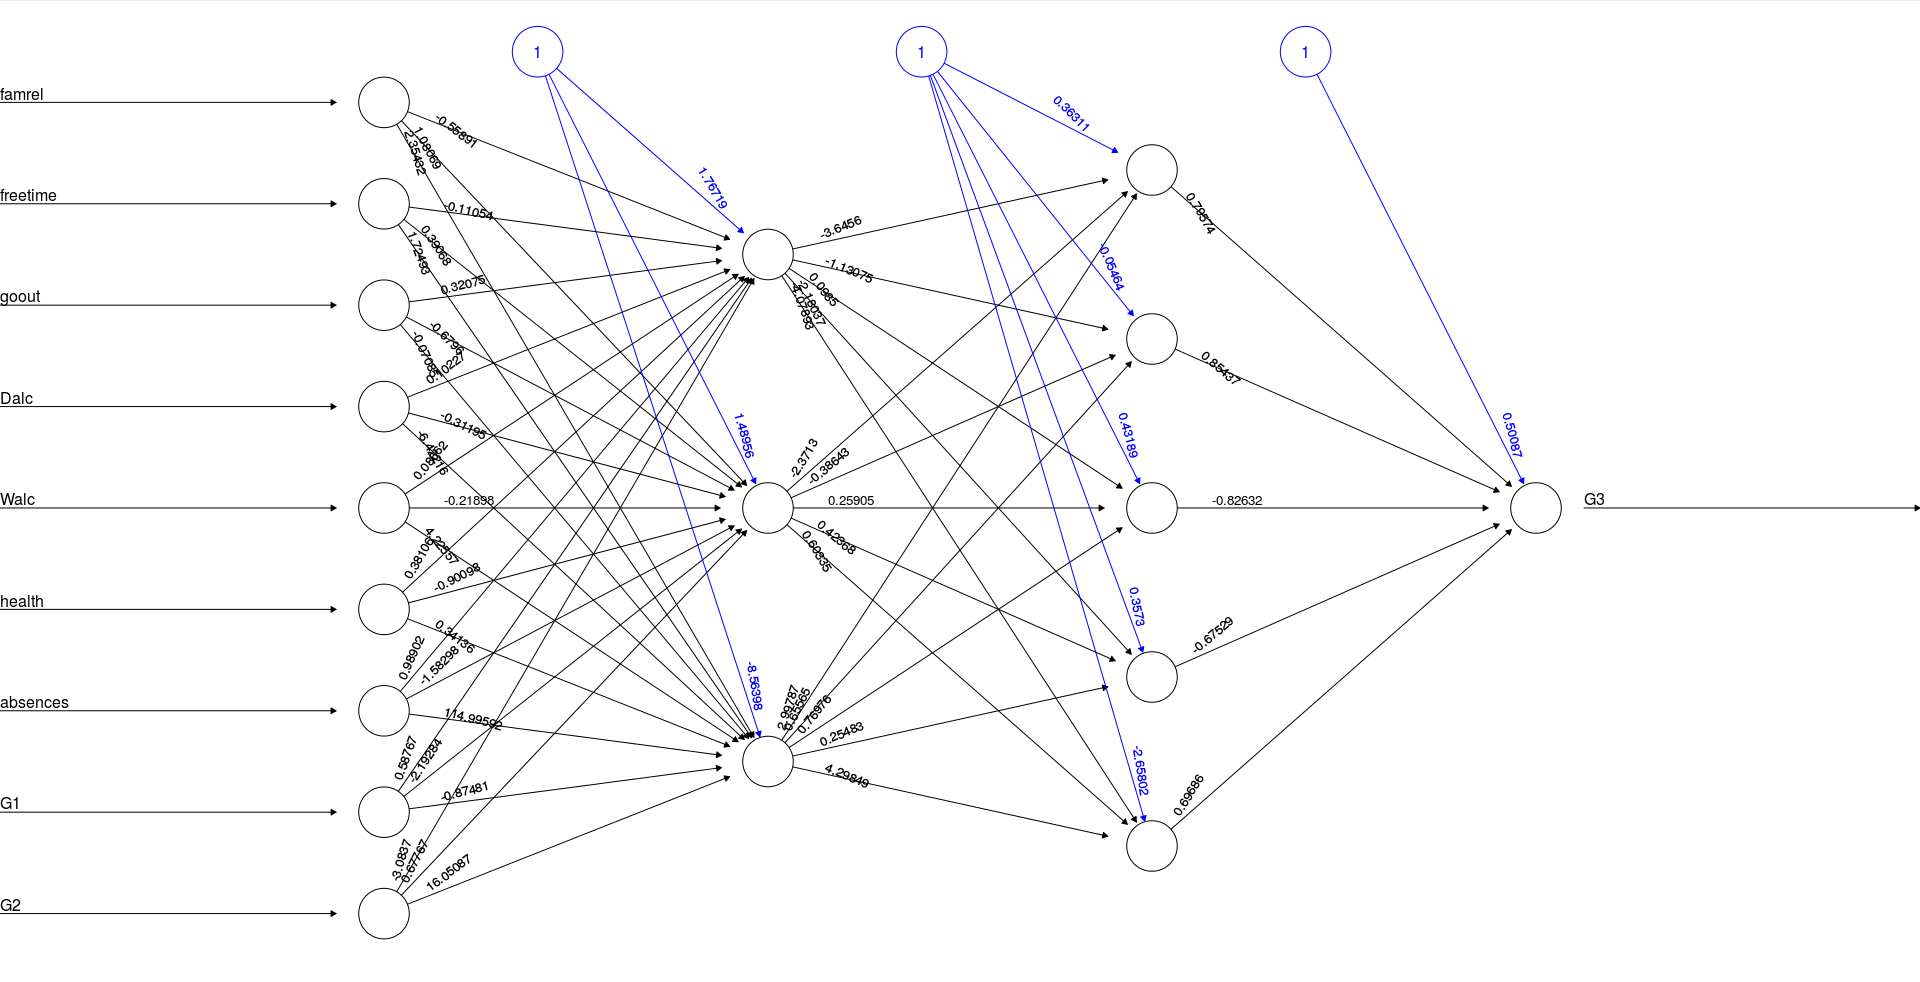
\includegraphics[width=\linewidth]{neural_net_math.png}
	\caption{Neural Network}
	\label{fig:neural-net}
\end{figure}

The proposed system is a predictive model that takes into account variables such
as performance in previous tests such as marks obtained in each internal test as well as
demographic variables such as health of the student and habits (both good and bad) of
the student as predictors. We also plan to add weights based on course dependency to
improve the system (as shown in Fig. \ref{fig:DAProjectSystemFlow}), however this integration 
is a future enhancement we look to add once we get an opportunity to work on data with respect to
PES University students.

The system finally looks to predict the grade the student is most likely to obtain using
each of the predictors.

We have taken two distinct predictive models to build the system. However,before
diving into each of these models that are very important components of the system, we
would like to first illustrate the basic workflow of the system.

		\subsection{Components}
The first component we would like to explain is that of extraction of prerequisite
weights given a course corpus using text analysis.

The first step in this section was to web scrape NPTEL course transcripts from the
NPTEL website. This was accomplished with a python script. We then used R and applied 
text analysis concepts such as stop-word removal, stemming and term document matrix 
on each of the transcripts. The next step involved defining a threshold and extracting 
all the words that occur greater than or equal to the value of the threshold defined.

This was done for each course and its corresponding prerequisites and set intersection
was applied to quantify percentage of prerequisite in each course. Visualisations for
term frequency for the courses Artificial Intelligence is shown in Fig. \ref{fig:ai-vis}.
However due to unavailability of PES University student performance data we were
unable to integrate the findings to our model. Thus this component is slated to be a future
enhancement to our system. The core of the system for this semester’s course project
lies in the predictive models built, namely, a linear model and a neural network
model for predicting student performance using the UCI Exam Performance dataset.
However the component involving text analysis allowed us to apply concepts of text
analysis learnt in this course and the work done will allow us to improve our model once
we get PES University Student Performance Data.

The second component we would like to discuss is the predictive models used to predict
student performance. We built a linear model as well as a neural network and
predicted student performance in Math and Portuguese based on the UCI Exam
Performance Dataset\cite{Lichman:2013}\cite{ref:4}.

We would like to first explain the neural network model used. The initial model was built
using R. The first layer took 9 input variables to the first layer. These variables are the
predictors which include previous grades (G1 and G2), the family relationship of the
student (famrel), the amount of free time the student gets, the amount the student goes
out,the alcohol consumption of the student (Dalc and Walc), the number of time the
student was about during the course (absences) as well as the overall health of the
student. The final prediction is that of predicted course outcome denoted by G3.
The neural network also has two hidden layers with 3 and 5 neurons respectively. A
visualisation of the neural network built and trained with respect to the math course
present in the UCI Exam Performance dataset is shown in Fig. \ref{neural-net}.
The black lines show the connections between each layer and the weights on each
connection while the blue lines show the bias term added in each step.

We also built deep neural network classifier using TensorFlow \cite{tensorflow2015-whitepaper} with
3 hidden layers with 10, 20 and 10 neurons. The models were validated with that present
in the paper “Using Data Mining to Predict Secondary School Student Performance “ by
P. Cortez and A. Silva and results we obtained which are discussed in Section \ref{expts-reslts}

We also built a linear model as for this particular problem of prediction for the purpose of comparison. The model was built with the same 9 predictors as that of the neural network as parameters with the final course performance outcome (G3) as the response variable.
Comparisons in terms of RMSE values of the models used as well as the models used
in Cortez et. al.\cite{ref:4} are discussed in the Section \ref{expts-reslts}.

	%--------------------------------------------------------------------------- Data  Sample----------------------------------------------------------------------------------
\begin{figure}
	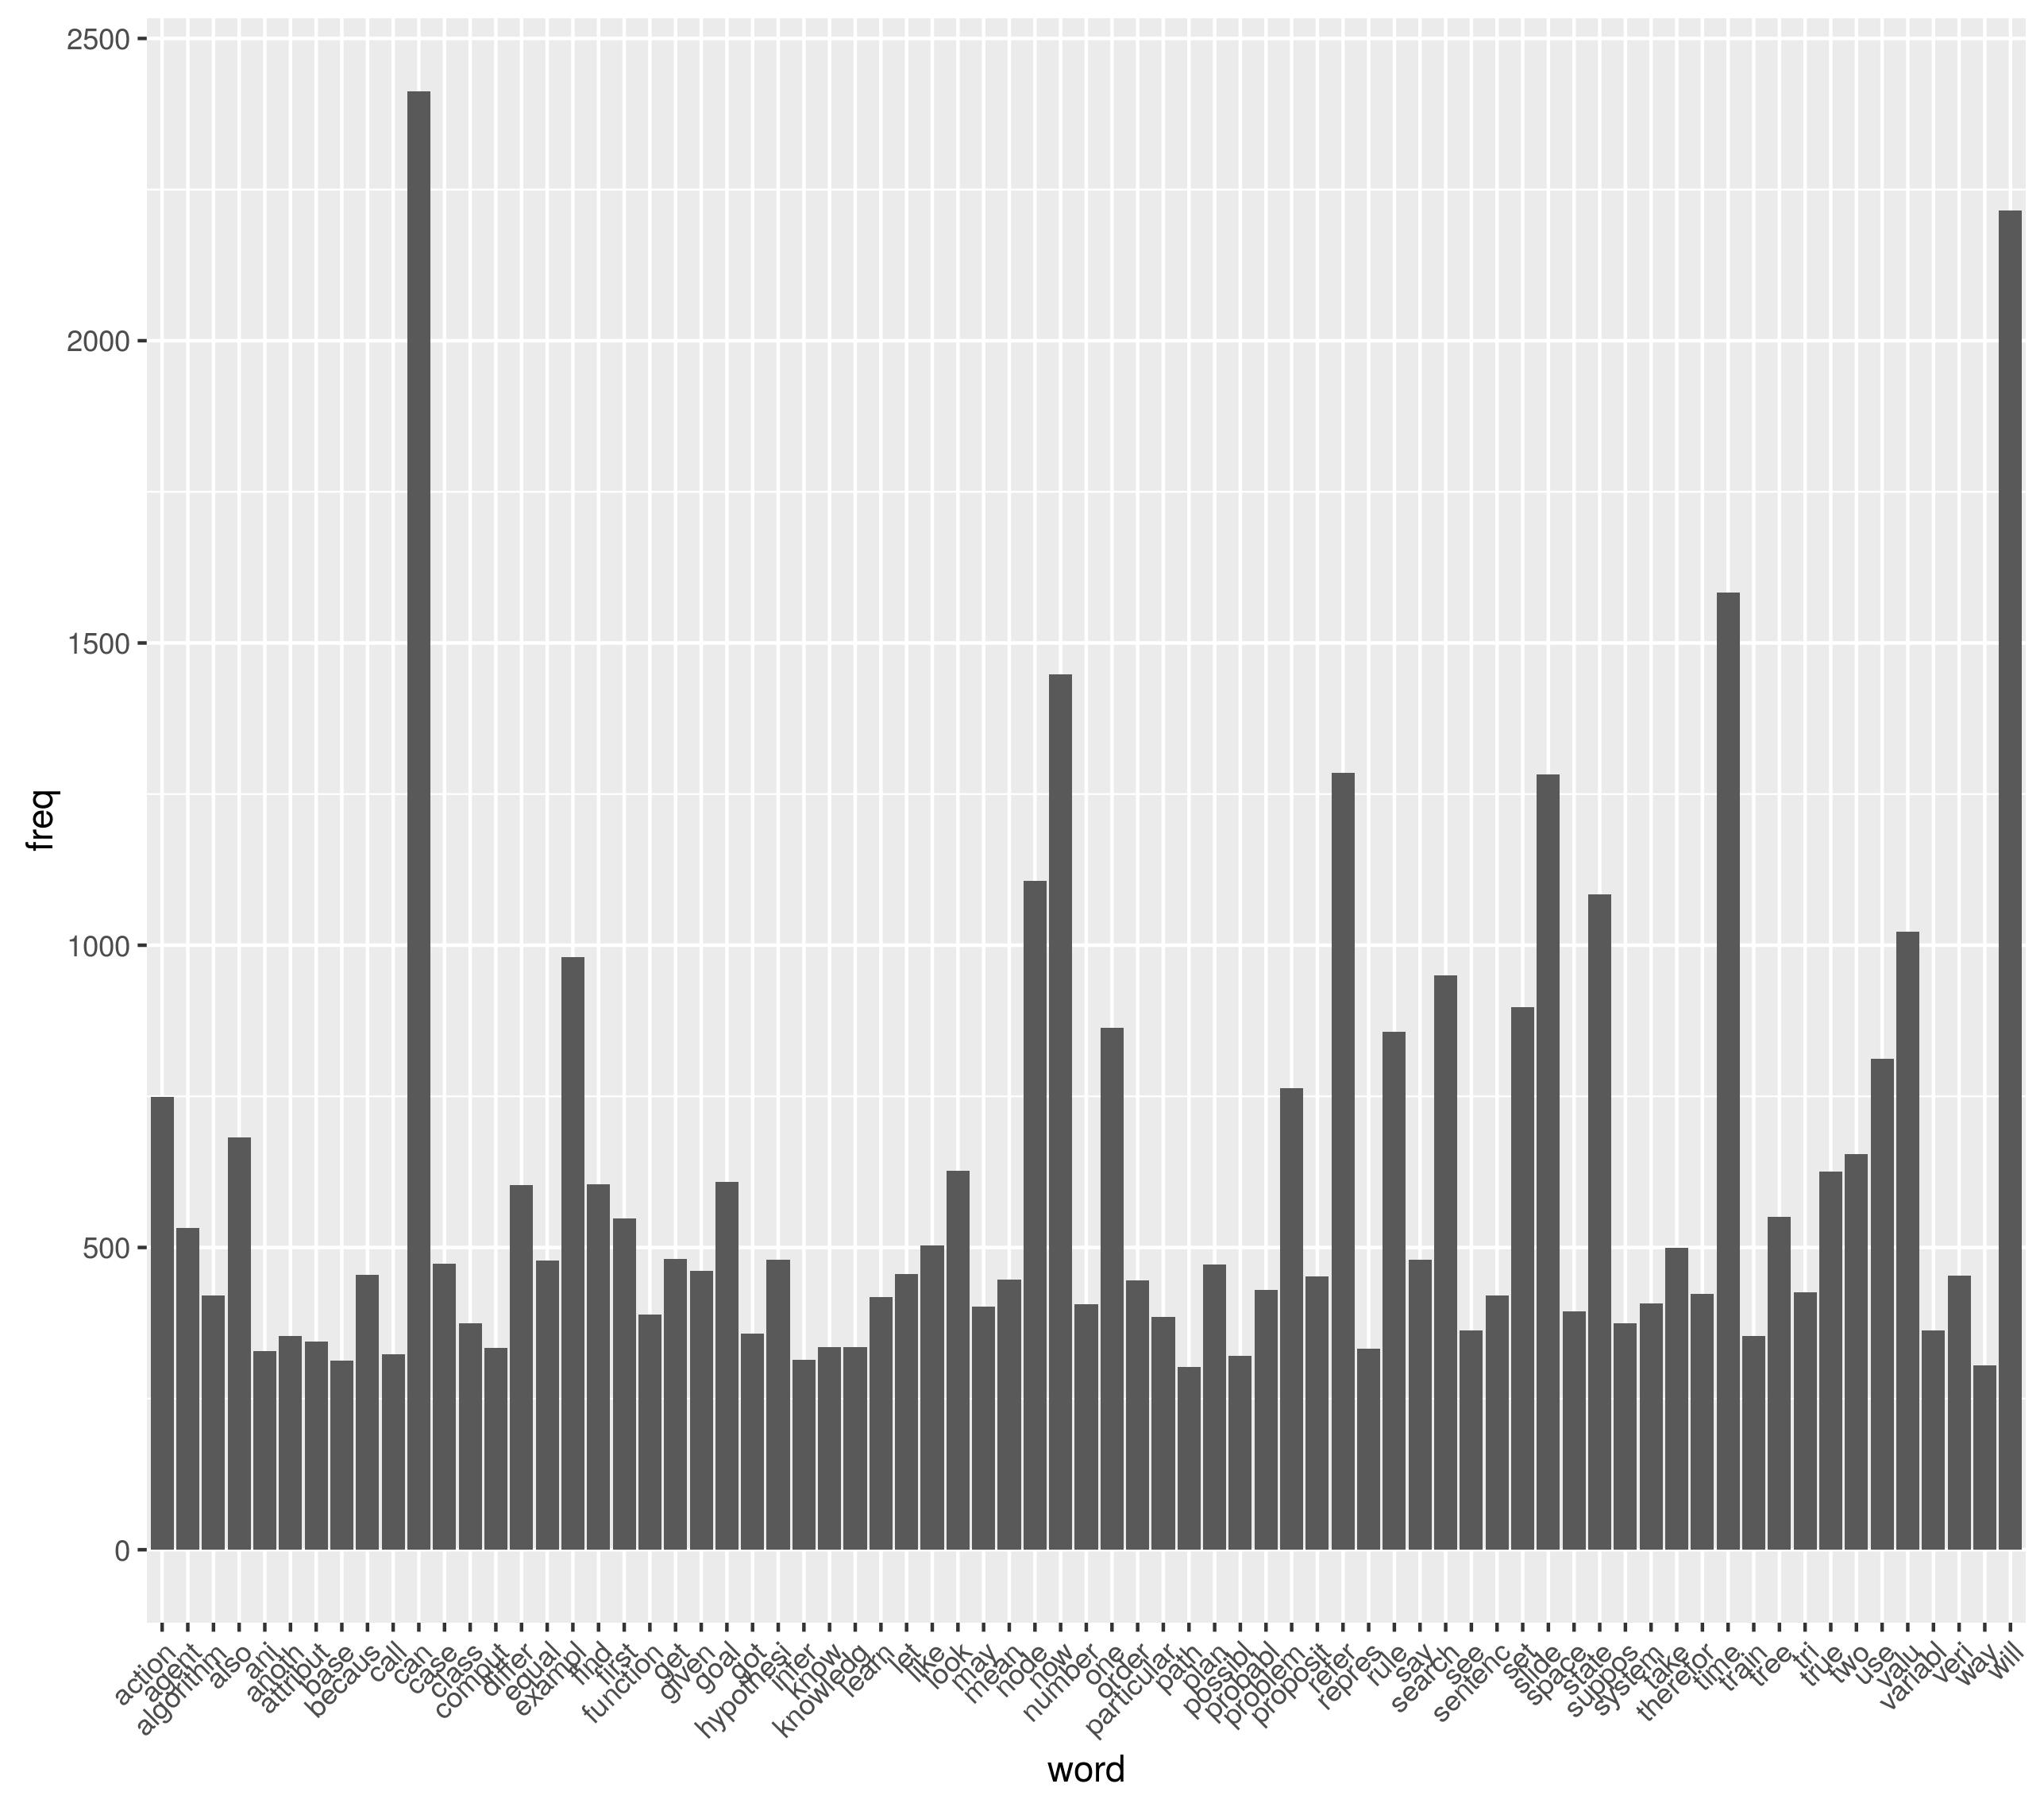
\includegraphics[width=\linewidth]{ai-vis.jpg}
	\caption{Term frequency visualisation of the course 'Artifical Intelligence'}
	\label{fig:ai-vis}
\end{figure}

	\section{Data Sample}

The dataset used in the project is the Student Performance dataset available from the UCI 
Machine Learning Repository. The UCI Machine Learning Repository is a collection of databases, 
domain theory, and data generators that are used by machine learning community for the empirical 
analysis of machine learning algorithms \cite{Lichman:2013}.

The data was collected in 2005-2006 from two public schools in the Alentejo region of Portugal. 
The data was built from two sources. The first - a questionnaire consisting of various multiple choice 
questions related to various factors that were expected to affect student performance according 
to Cortez et. al. \cite{ref:4}. These factors included information like weekday alcohol and 
weekend alcohol consumption, heath factors, previous class failures, etc. The second source of 
data were the schools' official student records which included their grades. The student records 
were in paper form. The data collection and integration was done by hand \cite{ref:4}.

The grading system is similar to our university's system. The assessment is carried out at three 
periodic intervals, and the last assessment is considered the final grade. The grading is done on a scale 
of 0 to 20, with 0 being the worst score possible, and 20 being a perfect score. The dataset includes 
the data for Mathematics and Portuguese Language subjects. The students in the Math and Portuguese dataset 
need not be the same \cite{ref:4}.

The questionnaire was answered by 788 students. Later, 111 answers were discarded due to lack of identification. 
Also, during the integration process, it was discovered that certain attributes were lacking in disciminative 
quality. For example, the field on their family income was left unanswered on most questionnaires, whereas close 
to everyone had a personal computer at home and lived with their families. These attributes were dropped \cite{ref:4}.

The number of records in the Math database is 395, and 695 for the Portuguese dataset.

The explanation of the attributes is given in Table \ref{table:attr-descr}.
	%--------------------------------------------------------------------------- Expts and reslts----------------------------------------------------------------------------------
	\section{Experiments and Results} \label{expts-reslts}

In the previous section we went into details with respect to the models that were built in the project to predict student performance. The UCI Student Exam Performance Dataset was split into training and test data. Training data consisted of 70\% of the dataset and the remaining 30\% of the dataset was used as test data. The neural network as well as the linear model were trained and tested. This was done for both the Math as well as the Portuguese courses present in the dataset. The performance of the models were very good. This is shown in Fig. \ref{fig:math-lm} and Fig. \ref{fig:math-nn} which plots the real vs predicted values using the Linear Model as well as the Neural Network model for the Mathematics course. Similar results were obtained for the Portuguese course as well.

\begin{figure}
	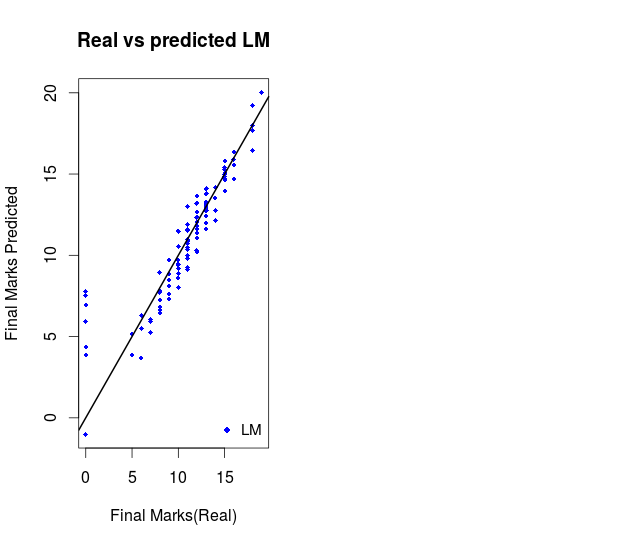
\includegraphics[width=\linewidth]{math_lm.png}
	\caption{Real vs. Fitted Values (Linear Regression Model)}
	\label{fig:math-lm}
\end{figure}
\begin{figure}
	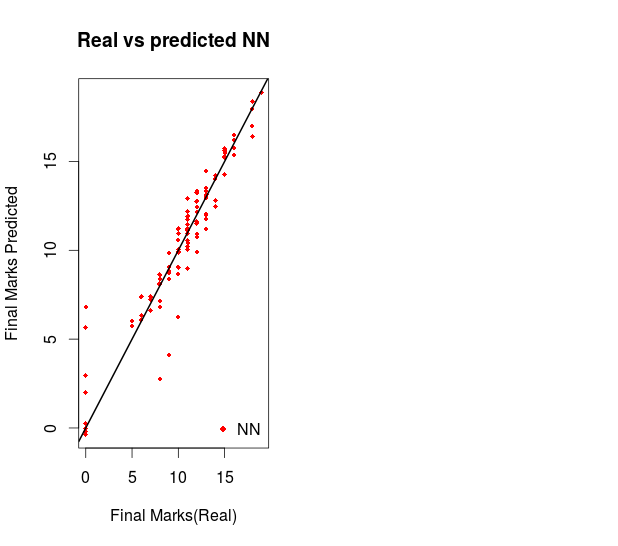
\includegraphics[width=\linewidth]{math_nn.png}
	\caption{Real vs. Fitted Values (Neural Network Model)}
	\label{fig:math-nn}
\end{figure}

We observed that both the linear model as well as the neural network performed in a similar fashion with the neural network having a slightly better RMSE value as compared to the linear model. In case of the Portuguese course, the linear model had a better RMSE value. The neural network we built using TensorFlow \cite{tensorflow2015-whitepaper} as described in the previous section had varying performance, as seen the table of our results (Tables \ref{table:res-mat} \& \ref{table:res-por}).

	\subsection{Validation of Models}
The next step was to validate our models. That is, we wanted to test how well it
performs as compared to a predictive model that has already been applied to the
dataset. This was done by comparing the RMSE values obtained by our models as compared to those obtained in the paper “Using Data Mining To Predict Secondary
School Student Performance” authored by P. Cortez and A. Silva.

% say the look at tables here
\begin{table*}[!t]
\renewcommand{\arraystretch}{1.3}
\caption{Results of Predictions for Mathematics (RMSE)}
\label{table:res-mat}
\centering
\begin{tabular}{|c c c|}
\hline
%header
\bfseries Linear Model & \bfseries Neural Network (two layer) & \bfseries Deep Neural Network (three layer)\\
\hline
%body
1.93 & 1.48 & 1.78 - 2.5\\
\hline
\end{tabular}
\end{table*}

\begin{table*}[!t]
\renewcommand{\arraystretch}{1.3}
\caption{Results of Predictions for Portuguese (RMSE)}
\label{table:res-por}
\centering
\begin{tabular}{|c c c|}
\hline
%header
\bfseries Linear Model & \bfseries Neural Network (two layer) & \bfseries Deep Neural Network (three layer)\\
\hline
%body
1.21 & 1.51 & 1.48 - 2.05\\
\hline
\end{tabular}
\end{table*}

Thus, the results obtained show that neural network models in some cases have 
obtained a better RMSE value. But most surprisingly, the linear model managed to perform better compared to most of the approaches used in Cortez et. al. \cite{ref:4}. This result provides us with a solid foundation to carry our research forward as with the addition of course dependency weights to our model which is our future enhancement we look to further improve the model and thus come one step closer to our aim of making an impact in the field of education through data analytics.

	%---------------------------------------------------------------------------Conclusion----------------------------------------------------------------------------------

\begin{table*}[!t]
\renewcommand{\arraystretch}{1.3}
\caption{Description of Attributes}
\label{table:attr-descr}
\centering
\begin{tabular}{|r || l|}
\hline
\bfseries Attributes & \bfseries Description \\
\hline\hline
school & student's school (binary: 'GP' - Gabriel Pereira or 'MS' - Mousinho da Silveira)\\
age & student's age (numeric: from 15 to 22)\\
address & student's home address type (binary: 'U' - urban or 'R' - rural)\\
famsize & family size (binary: 'LE3' - less or equal to 3 or 'GT3' - greater than 3)\\
Pstatus & parent's cohabitation status (binary: 'T' - living together or 'A' - apart)\\
Medu & mother's education (numeric: 0 - none, 1 - primary education (4th grade), 2 - 5th to 9th grade, 3 - secondary education or 4 - higher education)\\
Fedu & father's education (numeric: 0 - none, 1 - primary education (4th grade), 2 - 5th to 9th grade, 3 - secondary education or 4 - higher education)\\
Mjob & mother's job (nominal: 'teacher', 'health' care related, civil 'services' (e.g. administrative or police), 'at\_home' or 'other')\\
Fjob & father's job (nominal: 'teacher', 'health' care related, civil 'services' (e.g. administrative or police), 'at\_home' or 'other')\\
reason & reason to choose this school (nominal: close to 'home', school 'reputation', 'course' preference or 'other')\\
guardian & student's guardian (nominal: 'mother', 'father' or 'other')\\
traveltime & home to school travel time (numeric: 1 - $<$15 min., 2 - 15 to 30 min., 3 - 30 min. to 1 hour, or 4 - $>$1 hour)\\
studytime & weekly study time (numeric: 1 - $<$2 hours, 2 - 2 to 5 hours, 3 - 5 to 10 hours, or 4 - $>$10 hours)\\
failures & number of past class failures (numeric: n if 1 $\leq$ n $<$ 3, else 4)\\
schoolsup & extra educational support (binary: yes or no)\\
famsup & family educational support (binary: yes or no)\\
paid & extra paid classes within the course subject (Math or Portuguese) (binary: yes or no)\\
activities & extra-curricular activities (binary: yes or no)\\
nursery & attended nursery school (binary: yes or no)\\
higher & wants to take higher education (binary: yes or no)\\
internet & Internet access at home (binary: yes or no)\\
romantic & with a romantic relationship (binary: yes or no)\\
famrel & quality of family relationships (numeric: from 1 - very bad to 5 - excellent)\\
freetime & free time after school (numeric: from 1 - very low to 5 - very high)\\
goout & going out with friends (numeric: from 1 - very low to 5 - very high)\\
Dalc & workday alcohol consumption (numeric: from 1 - very low to 5 - very high)\\
Walc & weekend alcohol consumption (numeric: from 1 - very low to 5 - very high)\\
health & current health status (numeric: from 1 - very bad to 5 - very good)\\
absences & number of school absences (numeric: from 0 to 93)\\
\hline
\end{tabular}
\end{table*}

	\section{Conclusion}
In this project, we introduced a system to predict student performance. Through this system we hope to make an impact in a number of areas such as student counseling, elective selection, understanding student interest levels before course commencement among others. We built three predictive models and neural network had a better accuracy in terms of RMSE values than the values presented by Cortez et. al. \cite{ref:4}, and the neural network built using TensorFlow \cite{tensorflow2015-whitepaper} seems to perform better, albeit with a varying degree of how well it performs. Reduction of error in any field is important and thus this reduction of RMSE value through our work this semester provides a solid foundation to build a very accurate student education support system. We also showed that a number of demographic variables affect student performance and it is not just previous grades although previous grades do have a strong influence. Our future work involves quantifying percentage of pre requisites for each course and using the weights obtained to improve the system.

	%---------------------------------------------------------------------------Acknowledgment----------------------------------------------------------------------------------
	\section*{Acknowledgment}
We thank our professors from PES University who provided insight and expertise that greatly assisted the research, although they may not agree with all of the conclusions of this literature survey. We would like to show our gratitude to the Dr. Viraj Kumar, Professor, PES University,\\  Dr. Gowri Srinivasa, Professor, PESIT South Campus and \\ Prof. Shreekanth M. Prabhu , Professor, PES University for giving us this opportunity and sharing their pearls of wisdom with us.

	%---------------------------------------------------------------------------Contrib----------------------------------------------------------------------------------
	\section*{Contributions}
This project was very much a team effort. It was only with the efforts and entusiasm that we managed to complete the project to a satisfactorial level, despite the setbacks that we, as a team, suffered due to the non-availability of the data we needed to perform our original idea for analysis. All steps and work done in the project was a result of heated debates and discussion within the team.\\
Anush\IEEEauthorrefmark{1} was responsible for building our neural network models.\\
Sreedhar\IEEEauthorrefmark{2} was responsible for building the linear model, data sourcing, and implementing the simple two-layer neural network model. His work was mostly in R \cite{r}.\\
Sushrith\IEEEauthorrefmark{3} was responsible for performing text analytics on the course material using NLTK \cite{Loper02nltk:the} and Python, and also used the Deep Neural Network Classifier of TensorFlow \cite{tensorflow2015-whitepaper} to implement the three-layer deep neural network classifier.

\bibliography{ref}
\bibliographystyle{IEEEtran}
\end{document}
